\chapter{Automatic Speech Recognition}

\section{Co je to ASR}

ASR (Automatic Speech Recognition) je teoretický model, založený na pravděpodobnostních vlastnostech akustických pozorování, který formalizuje převod mluveného slova do textu. Přeneseně se takto označují i konkrétní systémy a implementace, které tohoto modelu využívají. 

Ultimátním cílem  je získat systém, který bude v reálném čase převádět přirozenou lidskou řeč na text se stoprocentní úspěšností pro všechna slova, nezávisle na zkreslení vstupních zařízení, okolním ruchu, nebo přízvuku mluvčích. Již v minulosti ASR systémy dosahovaly i kolem devadesátiprocentní úspěšnosti \cite{jelinek_1976}. Nyní lze nalézt systémy s úspěšností i větší, hlavně však systémy optimalizovanější a výkonnější.

\section{Postup rozpoznávání}

\begin{figure}[h]
	\centering
	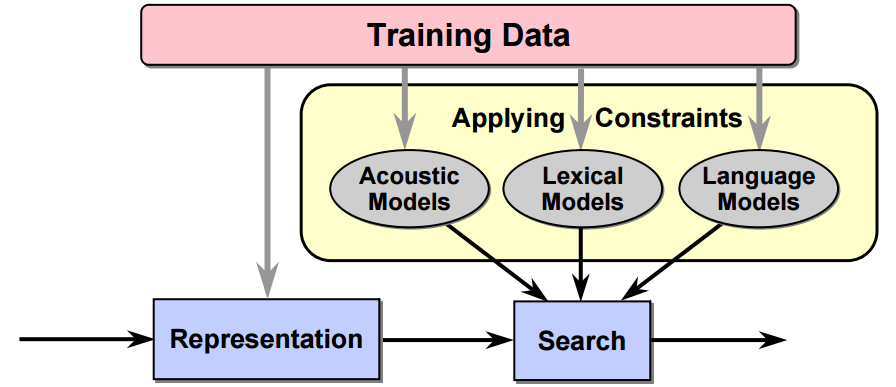
\includegraphics[width=140mm]{img/asr_process.png}
	\caption{Hlavní součásti ASR systému \cite{mit_asr_2003}}
	\label{fig:asr_process}
\end{figure}

Obrázek \ref{fig:asr_process} ukazuje, že samotný návrh systému je poměrně přímočarý.
\\\\*
Zásadními milníky systému jsou:

\begin{itemize}
\item Jak zpracovat signál?
\item Jak se popasovat s omezeními?
\item Jak nalézt optimální výstup?
\end{itemize}

\section{Reprezentace a zpracování signálu}

Pro reprezentaci a zpracování signálu se běžně využívají dva druhy analýzy -- analýza pomocí {\sl discrete-time} Fourierovy transformace (\nom{DTFT}{Discrete-Time Fourier Transform}) a Cepstrální analýza (\nom{CA}{Cepstral Analysis}).

\subsection{Fourierovská analýza}

{\sl {\sl Discrete-time} Fourierova transformace} je vztah:
\begin{align}
	\label{eq:dtft}
	X(e^{j\omega}) &= \sum\limits_{n=-\infty}^{+\infty} x[n] e^{-j\omega n}\\
	          x[n] &= \frac{1}{2\pi} \int_{-\pi}^{\pi} X(e^{j\omega})e^{j\omega n} d\omega
\end{align}
jemuž pro konvergenci postačuje podmínka:
\begin{equation}
	\label{eq:dtft_conv}
	\sum\limits_{n=-\infty}^{+\infty} |x[n]| < +\infty
\end{equation} 

Ačkoli je $x[n]$ diskrétní, $X(e^{j\omega})$ je spojitá, $2\pi$-periodická a pro její dualitu platí:
%
\begin{align}
	\label{eq:dtft_d}
	          y[n] &= x[n] * h[n]\\
	Y(e^{j\omega}) &= X(e^{j\omega})H(e^{j\omega})
\end{align}
%
a
%
\begin{align}
	          y[n] &= x[n]w[n]\\
	Y(e^{j\omega}) &= \frac{1}{2\pi} \int_{-\pi}^{\pi} W(e^{j\theta})X(e^{j(\omega - \theta)})d\theta
\end{align}

V důsledku můžeme zavést {\sl short-time} fourierovskou analýzu (\nom{STFA}{Short-Time Fourier Analysis} -- Short-Time Fourier Analysis) jako:
%
\begin{equation}
	\label{eq:stfa}
	X_n(e^{j\omega}) = \sum\limits_{m=-\infty}^{+\infty} w[n-m]x[m]e^{-j\omega m}
\end{equation}
%
a v případě, že $X(e^{j\omega})$ representuje DTFT signálu, který pokračuje i mimo okno brané v potaz (nebo je tam konstantní nula), můžeme psát, že:
%
\begin{equation}
	\label{eq:stfa_f}
	X_n(e^{j\omega}) = \frac{1}{2\pi} \int_{-\pi}^{\pi} W(e^{j\theta})e^{j\theta n}X(e^{j(\omega + \theta)})d\theta
\end{equation}

\subsection{Cepstrální analýza}

Původně CA vznikla jako nástroj analýzy časového rozvoje seismických signálů vzniklých zemětřeseními, či explozemi. Měla pomoci nalézt především hloubku generátoru seismických signálů analýzou odezvy těchto signálů \cite{bogert_1963}.

CA využívá předpokladu, že signál je výstup lineárního časově invariantního (\nom{LTI}{Linear Time-Invariant} -- Linear Time-Invariant) systému; tedy že je to konvoluce vstupu a impulsové odezvy. Pokud se chceme zabývat charakterizací tohoto modelu, musíme projít procesem dekonvoluce. A CA je právě postup, využívaný pro takovouto LTI dekonvoluci \cite{tohkura_1987}.

Vezmeme-li v potaz pozorování, že:
%
\begin{equation}
	\label{eq:ca_obs}
	x[n] = x_1[n] * x_2[n] \iff X(z) = X_1(z) X_2(z)
\end{equation}
%
a vyjádříme-li komplexní logaritmus $X(z)$ jako:
%
\begin{equation}
	\label{eq:ca_l}
	\widehat{X}(z) = \log X(z) = \log X_1(z) + \log X_2(z)
\end{equation}
%
pak pokud je tento logaritmus jednoznačný a $\widehat{X}(z)$ je validní z-transformace, jsou nové konvolvované signály aditivní v této nové cepstrální doméně:
%
\begin{equation}
	\label{eq:ca_xl}
	\widehat{x}(n) = \widehat{x}_1(n) + \widehat{x}_2(n)
\end{equation}

Pokud se navíc omezíme na jednotkovou kružnici $z = e^{j\omega}$, pak cepstrální transformací označujeme:
%
\begin{equation}
	\label{eq:ca_f}
	\widehat{X}(e^{j\omega}) = \log |X(e^{j\omega})| + j \arg X(e^{j\omega})
\end{equation}

\section{Zdroje omezení mluvené komunikace}

Při předávání informace mluvenou řečí může běžně docházet ke zkreslení řečené informace díky několika nepříjemným faktorům, které mohou (a budou) ASR systému působit nepříjemnosti. Těmto omezením se nelze vyhnout, proto jsou ASR systémy nuceny brát v potaz rozličné nepřesnosti a snažit se tyto eliminovat.

Práci už tak nepříjemnou nezlehčuje ani fakt, že omezení nejsou konstantně daná; lze je pouze taxonomizovat a obcházet.
\\\\*
Patří sem například:

\begin{itemize}
\item Akustická omezení -- lidský hlasový aparát trpí, jako každý jiný komplexní systém, také svými neduhami
\item Fonetická omezení -- \uv{kolemjdoucí paní} - \uv{kolem jdou cíp a ní}
\item Fonologická omezení -- například splynutí \uv{s} a \uv{š} do jednoho dlouhého fonému - \uv{lezeš shora}
\item Fonotaktická omezení -- kupříkladu zjednodušení konsonantických shluků u menších dětí (\uv{uličnice} - \uv{ulitite}), nebo nesmyslná, rádoby přejatá slova (\uv{sympathetic} - \uv{sympatetický})
\item Syntaktická omezení -- \uv{jedu na výlet do Českých Budějovic} - \uv{Českých výlet na Budějovic jedu do}
\item Sémantická omezení -- \uv{zapal sirku} - \uv{zapal si ruku}
\item Lexikální omezení -- \uv{šuplánek} ani \uv{niplavý} nejsou česká slova
\end{itemize}

a mnohá další.

\section{Modelování systému}

V ASR procesu se stroj pokouší nalézt co možná nejlepší shodu získaného signálu (reprezentace přirozené řeči) a posloupnosti písmen (slov, vět). Abychom něčeho podobného mohli dosáhnout, musíme navrhnout dostatečně komplexní a efektivní model, který nám (a našim strojům) dá do ruky nástroj pro formulaci problému, jeho porozumění a metodologii potřebnou k jeho rozlousknutí.

\subsection{Maximum a Posteriori formulace}

Tato formulace se \uv{pokouší nalézt nejpravděpodobnější sekvenci slov $W^*$ při daném akustickém vstupu $A$} \cite{jelinek_2010}. \nom{MAP}{Maximum a Posteriori} přístup \cite{bahl_jelinek_1983} lze typicky vyjádřit jako:

\begin{equation}
	\label{eq:map}
	W^* = \arg \max_{W} P(W|A)
\end{equation}

\newtheorem{t:bayes}{Věta}
\begin{t:bayes}
Bayesova věta \\
Pro náhodné nezávislé jevy $X$ a $Y$ platí:
\begin{equation}
	\label{eq:bayes}
	P(X|Y) = \frac{P(Y|X) P(X)}{P(Y)}
\end{equation}
\end{t:bayes}

Za použití \ref{eq:bayes} můžeme upravit pravou stranu rovnosti \ref{eq:map}, čímž dostaneme vztah:

\begin{equation}
	\label{eq:map2}
	W^* = \arg \max_{W} \frac{P(A|W) P(W)}{P(A)}
\end{equation}\
%
kde $P(A|W)$ je nazývána charakteristikou akustického modelu (\nom{AM}{Acoustic Model} -- Acoustic Model) a $P(W)$ charakteristikou jazykového modelu (\nom{LM}{Language Model} -- Language Model). Jelikož $P(A)$ je konstantní vůči této maximalizaci, můžeme se jí hladce zbavit a psát:

\begin{equation}
	\label{eq:map3}
	W^* = \arg \max_{W} P(A|W) P(W)
\end{equation}

\subsection{Jazykové modely}

Modelování jazyka poskytuje nástroj, jak odlišit slova a fráze, které zní podobně, či stejně (homografy, homofony, homonyma). Kupříkladu v americké angličtině jsou věty \uv{recognize speech} a \uv{wreck a nice beach} sémanticky diametrálně odlišné, foneticky jsou to však věty téměř homofonní. 

Jelikož vyhledávání je v drtivé většině případů pouze jednosměrné, můžeme pravděpodobnost posloupnosti slov $W = w_1, \dots, w_n = w^n_i$ vyjádřit pomocí řetízkového pravidla a napsat jako:

\begin{equation}
	\label{eq:lm}
	P(w^n_i) = \prod\limits_{i=1}^n P(w_i|w^{i-1}_1)
\end{equation}

Protože sekvence $W$ může mít jednoduše příliš mnoho prvků a navíc pravděpodobnost $P(w_i)$ nemusí nutně záviset na úplně celé historii $h_i = w_1^{i-1}$, slučujeme $h_i$ do tříd ekvivalence $\Phi (h_i)$, čímž dospíváme k:

\begin{equation}
	\label{eq:lm_ec}
	P(w^n_i) \approx \prod\limits_{i=1}^n P(w_i|\Phi (h_i))
\end{equation}

Jak možno nahlédnout, pro kvalitní odhad je kritické určit dobré zobrazení $\Phi$. Čím lepší návrh tohoto zobrazení, tím lepší informaci získáme o $w_i$, využívaje historie $\Phi (h_i)$.

Zde nastupují na scénu {\sl n-gram} modely \cite{byeo_2012}\cite{masa_1997}, které v tomto případě zavádějí $n-1$ předchozích slov pro reprezentaci historie, tj. $\Phi (h_i) = w_{i-(n-1)}^{i-1}$, čímž získáme:

\begin{equation}
	\label{eq:lm_ec}
	P(w^n_i) \approx \prod\limits_{i=1}^n P(w_i|w_{i-(n-1)}^{i-1})
\end{equation}

Například uvážíme-li {\sl bigram} ({\sl n-gram}, $n = 2$), pravděpodobnost věty \uv{České Budějovice jsou krásné město}, tj. posloupnosti slov:
%
\begin{align*}
	W = Ceske, Budejovice, jsou, krasne, mesto
\end{align*}
%
lze vyjádřit jako:

\begin{align*}
	P(W) =&~P(Ceske|<\! start\!>)P(Budejovice|Ceske)\\
	      &~P(jsou|Budejovice)P(krasne|jsou)\\
	      &~P(mesto|krasne)P(<\! konec\!>|mesto)
\end{align*}

Pravděpodobnosti $P(w_i|w_{i-(n-1)}^{i-1})$ můžeme dále odečíst z natrénovaných dat vztahem:

\begin{equation}
	\label{eq:lm_est}
	P(w_i|w_{i-(n-1)}^{i-1}) = \frac{c(w_{i-(n-1)}^{i})}{c(w_{i-(n-1)}^{i-1})}
\end{equation}
\\*
kde $c(\xi_p^q)$ představuje četnost výskytů posloupnosti $\xi_p^q$.

Kvůli možné nepřiměřené míře řídkosti dat je nasnadě uvážit možnost, že dělitel $c(w_{i-(n-1)}^{i-1})$ bude nulový, tedy že posloupnost ještě nebyla natrénována. 

Pro eliminaci těchto faktorů lze využít například některý z vyhlazovacích algoritmů (Jelinek-Mercer \cite{jelinek_1980}, Katz \cite{katz_1987}, Good-Turing \cite{church_1991}), nebo drobně pozměnit paradigma a přizvat na pomoc neuronové sítě \cite{chienli_2013}.

Buď jak buď, {\sl bigramy} stále zachovávají svou pozici v modelování jazyka --- lze je jednoduše zakomponovat do Viterbiho vyhledávání \cite{goblirsch_1996} --- a {\sl trigramy} ({\sl n-gram}, $n=3$) pokračují v bytí dominantním modelem.

\subsection{Akustické modely}

Modelováním akustiky můžeme naopak získat nástroj pro zachycení a vypořádání se například s akustickým šumem, se zkreslením vstupního zařízení, či s netradičním přízvukem mluvčího.

Akustický model statisticky reprezentuje zvuky, jenž poskládány dohromady tvoří vyřčené slovo. Každé takovéto statistické reprezentaci může být přiřazena nálepka ji reprezentující (běžně foném). Aby model mohl poskytovat rozumné výsledky, je potřeba jej nejprve natrénovat na nějakém jazykovém korpusu, například pro tento účel lze využít Baum-Welchova trénovacího algoritmu \cite{han_2003}.

Skryté Markovovy modely (\nom{HMM}{Hidden Markov Model}s -- Hidden Markov Models) \cite{poritz_1988} jsou jednou z možných interpretací akustického modelu (jiné interpretace mohou zahrnovat například neuronové sítě \cite{kingsbury_2009}, nebo {\sl dynamic time warping} \cite{tarar_2010}).

Při použití HMMs jeden HMM reprezentuje každý foném, slova vznikají konkatenací menších HMMs, věty na oplátku konkatenací těchto HMMs a tak dále.

Proč zrovna \uv{skrytý} Markovův model? Tento název vychází z definice \uv{skrytého} Markovova procesu (\nom{HMP}{Hidden Markov process} -- Hidden Markov process), který popíšeme za pomoci kolegů Alibaby a Rychlonožky a jejich uren. 

Vezměme myšlenkový experiment, kde v místnosti za zavřenými dveřmi žije Alibaba se třemi svými urnami $u_1, u_2, u_3$. Každá urna obsahuje známou množinu kuliček $\{k_{u_i}\}_1^n$, kde platí $(\forall u \in \{u_1, u_2, u_3\})(\forall j \in \{1,\dots,n\})(k_{uj} \in \{c_1,\dots,c_n\})$, tedy každá kulička z každé urny je jedné z barev $c$. Alibaba bude nyní ďábelským způsobem tahat kuličky z uren, a sice tak, že $l$-tou kuličku $K_l$  vytáhne náhodně a pouze s ohledem na $K_{l-1}$. Tomuto procesu se říká Markovův proces. Jelikož Alibaba na běhání nikdy nebyl, dá taženou $K_l$ Rychlonožkovi, který vyběhne ven dveřmi a složí $K_l$ k nohám nezávislého pozorovatele, hned vedle kuličky $K_{l-1}$ do řady.

Pozorovatel sice zná složení kuliček v urnách, ale nemá ani tušení, co se za dveřmi děje --- Markovův proces je skrytý --- takže může pouze smutně sledovat sekvenci kuliček, rodící se mu pod nohama. Po $1<m<n$ tazích a Rychlonožkovo sprintech bude mít pozorovatel v zorném poli posloupnost kuliček $K_1^m$. Problém ale nastává, chce-li pozorovatel určit z jaké urny byla tažena $K_m$. Ani v případě, že $(\exists i \in \{1, 2, 3\})(K_1^m \subseteq \{k_{u_i}\}_1^m)$ si totiž nemůže být jist.

Nicméně, pozorovatel se může alespoň pokusit odhadnout pravděpodobnost, že $K_m$ byla z urny $i$.

\subsection{Lexikální modely}

Lexikální modely popisují vztah mezi jednotkami akustickými (fonémy -- části slova mluveného, popsané akustickými modely) a lexikálními (lexémy -- jazykový odraz reality na vědomí). 

Pro ilustraci lexému vezměme slova \uv{ředkvička} a \uv{ředkvičky}; mají rozdílné gramatické a sémantické významy (singulár a plurál téhož), lexikální význam je ale stejný (malý, načervenalý, jedlý kořen). 

Jednou z výzev navrhování ASR systému je popsat tyto vztahy pro jazyk, kde lexikální příznaky nejsou zcela zřejmé. Jak ale \cite{rasipuram_2014} uvádí, pro standardní stochastické HMM ASR systémy existuje lexikální model deterministický, tj. existuje bijektivní zobrazení mezi trénovanými HMMs a lexémy.

Pro jazyky obtížné, s ne zcela formálními lexikálními příznaky, lze lexikální model odvodit z některého lexikálního modelu již známého -- aplikací známého modelu na nový jazyk a jeho postupnou adaptací.

Zavedeme-li $\Theta = \{\Theta_A, \Theta_L\}$ množinu parametrů akustických a jazykových modelů, kde $\Theta_A = \{\theta_a, \theta_pr, \theta_l\}$ jsou parametry akustického modelu, respektive lexikonu, respektive lexikálního modelu, můžeme s využitím \ref{eq:map} a \ref{eq:bayes} rozvést:

\begin{align}
	\label{eq:lm}
	W^* &= \arg \max_W P(W|A, \Theta)\\
	    &= \arg \max_W \frac{P(A|W, \Theta_A)P(W|\Theta_L)}{P(A|\Theta)}\\
	    &= \arg \max_W P(A|W, \Theta_A)P(W|\Theta_L)
\end{align}

Hledání nejpravděpodobnější sekvence $W^*$ pro akustický vstup $A$ pak můžeme díky lexikálnímu modelování transformovat na problém hledání nejpravděpodobnější posloupnosti stavů $Q^*$:

\begin{align}
	\label{eq:lm_state}
	Q^* &= \arg \max_Q P(Q,A|\Theta)\\
	    &= \arg \max_Q \prod\limits_{t=1}^T p(a_t|q_t = l^i, \Theta_A) P(q_t = l^i|q_{t-1} = l^i, \Theta)\\
	    &= \arg \max_Q \sum\limits_{t=1}^T (\log p(a_t|q_t = l^i, \Theta_A) + \log P(q_t = l^i|q_{t-1} = l^i, \Theta)) 
\end{align}
%
kde $T$ je celkový počet uvažovaných oken, $Q = \{q_1,\dots,q_t\}$ jde přes všechny posloupnosti možných HMM stavů, $q_t \in \{l^1,\dots,l^i,\dots,l^I\}$ a $I$ značí počet lexémů. Obvykle je výraz $\log p(a_t|q_t = l^i, \Theta_A)$ označován jako lokální emisní skóre (\nom{LES}{Local Emission Score} -- Local Emission Score) a výraz 
$\log P(q_t = l^i|q_{t-1} = l^i, \Theta)$ jako přechodové skóre (\nom{TS}{Transition Score} -- Transition Score).